\section{Cryogenic System}
\label{sec:cryostat}

The use of large quantities of highly-purified liquid argon as a detector medium in MicroBooNE requires a sophisticated cryogenic infrastructure that can maintain stable operations for years at a time.  Not only must the purity of the liquid argon be maintained, but the pressure and temperature gradients within the \lartpc active volume must be tightly controlled as the drift velocity of electrons is dependent on these quantities.  A customized cryogenic system that serves these purposes has been built, and the requirements for this system are shown in table \ref{tab:cryoreq}.

% Requires the booktabs if the memoir class is not being used
\begin{table}[!htb]
   \centering
    \caption{Primary design requirements for MicroBooNE cryogenic and purification systems.} 
    \begin{tabular}{lll} % Column formatting, @{} suppresses leading/trailing space
    \hline
    Parameter & Value & Motivation\\
    \hline
      Argon purity    & $<$100 ppt O$_2$ & MIP identification at longest drift\\
      Argon purity    & $<$2 ppm N$_2$ & Scintillation light output\\
      LAr Temperature gradient & $<$1$^\circ$ K & Drift-velocity uniformity\\
      LAr recirculation rate & 1 volume change/day & Maintain purity\\
      Cryostat heat load & $<$15 W/m$^2$ & Minimize convection currents and bubbles\\
      Cryogenic capacity & 10 kW & Capacity to deal with expected heat load\\
      Cryostat maximum pressure & 30 psig & Determines relief sizing\\
            \hline
   \end{tabular}
   \label{tab:cryoreq}
\end{table} 

The MicroBooNE cryogenic system is represented in figure \ref{fig:cryogenics}.  The central component of the system is a cryostat that houses the complete \lartpc and light-collection detector systems.  The cryostat is supported by three major subsystems: the argon purification system, the nitrogen refrigeration system, and the controls and monitoring system.  These systems each represent the next generation of \lartpc cryogenic system after the Liquid Argon Purity Demonstrator (LAPD)~\cite{Adamowski:2014-LAPD} and make considerable use of the expertise gained during the design and implementation of that apparatus.  %The LAPD was the first test stand to show that a large volume of liquid argon could be purified of electronegative contaminants without first evacuating the cryostat and still obtain electron lifetimes of $6$~ms and higher. 

\begin{figure}
\centering 
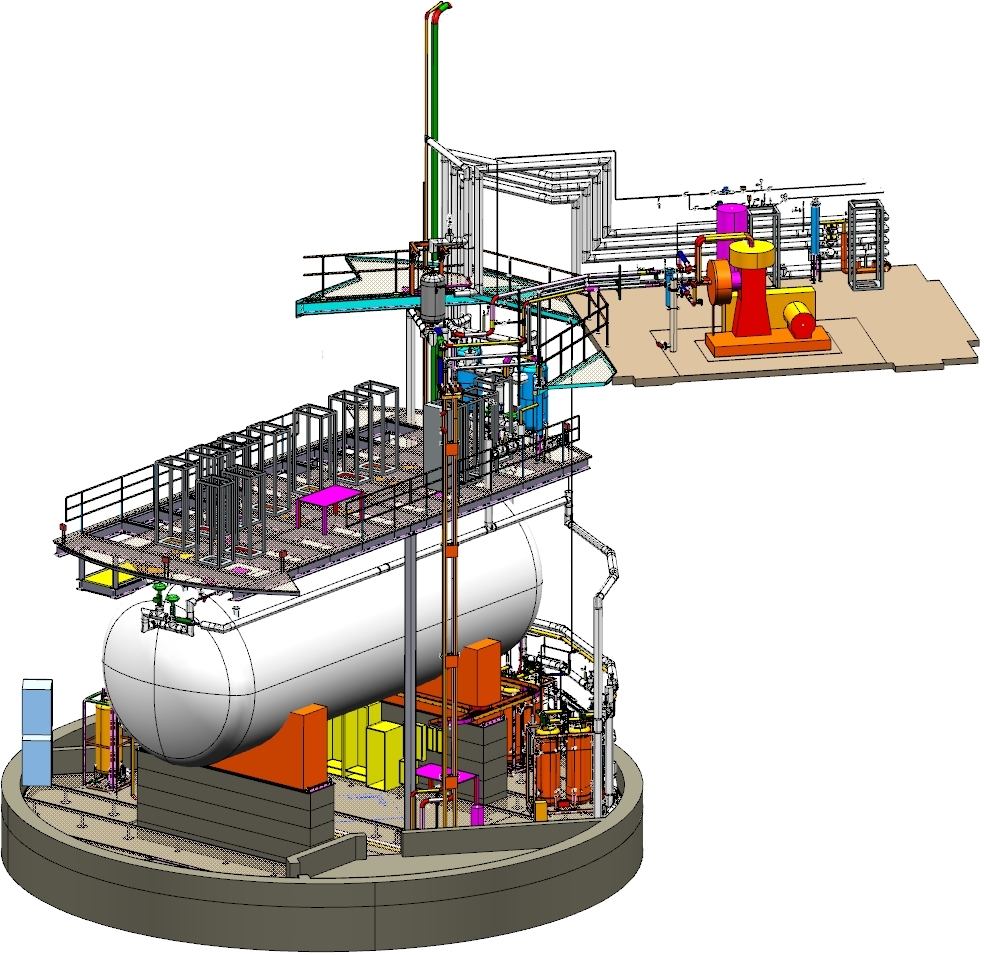
\includegraphics[width=0.95\textwidth]{figures/FULL-ASSY-1.jpg}
\caption{Three-dimensional renderings of the MicroBooNE cryogenic system installed at LArTF.}
\label{fig:cryogenics}
\end{figure}




\subsection{Cryostat Design Overview}

Three major components make up the MicroBooNE cryostat: a stainless steel (type 304) vessel to contain the liquid argon and all the active detector elements, front and rear supports to carry the weight of the fully loaded cryostat, and foam insulation covering the cryostat outer surfaces.  The foam insulation serves to reduce heat input from the ambient environment to a sufficiently low level to prevent large temperature gradients and boiling of the liquid argon. The cryostat and the cryogenic systems are designed to achieve the high-purity liquid argon needed to allow ionization electrons to drift to the anode wires with low probability of capture, and the high degree of thermal homogeneity needed to avoid the introduction of non-constant drift velocities for the ionization electrons. Finally, the outer diameter of the vessel is designed to be the maximum standard size for over-the-road transport.


Ionization electrons must not be significantly attenuated, via attachment to electronegative contaminants in the liquid argon, as they drift up to 2.5~m across the active volume. This dictates that the argon be kept free of electronegative contaminants to the level of 100 parts-per-trillion (ppt). The cryostat is designed to minimize outgassing (desorption) and to avoid leakage and diffusion of air into the system. This requirement imposes strict quality assurance demands on all welds for penetrations into the cryostat and on cleaning and handling procedures for the finished vessel.  Achieving the required level of purity is accomplished with a purification system, described in section~\ref{sec:purification}, that removes electronegative contaminants from the argon during the initial fill and those introduced over time by leaks and outgassing of system components.

The electron drift velocity ($v_{d} = 1600$~m/s at an electric field of 500 V/cm, with a liquid argon temperature dependence $\Delta v_{d}/v_{d} = -0.019\Delta T$) must remain constant in magnitude and direction throughout the active liquid argon volume to avoid distortion of the mapping of drift time into the position along the drift ($\hat{x}$) direction. This requirement limits the allowable temperature variations of the liquid argon to less than 0.1~K and the laminar and turbulent flow rate of liquid argon to less than 1~m/s. These requirements limit fractional errors in velocity, and therefore in the drift-coordinate determination, to be less than 0.1\%. The constraints on constancy of drift velocity affect the design by imposing limits on the acceptable heat flux through the insulation.

The cryostat is constructed to the latest American Society of Mechanical Engineers (ASME) boiler code requirements~\cite{pressure:1316452} and features a single-walled construction, cylindrical shape, and domed caps closing each end, as shown in figure~\ref{fig:cryostat-drawing}. One end was removed for installation of the active detectors, welded back in place upon completion of that task, and then recertified to the ASME code requirements.  Upon installation of the sealed cryostat in its final location at the Liquid Argon Test Facility (LArTF), 16 inches of spray-on, closed cell, Polyurethane insulation was applied to the exterior of the cryostat, as shown in figure~\ref{fig:cryostat-foam}.  At LArTF, to avoid ground loops that could interfere with the \lartpc signals, the cryostat vessel is grounded in only one place, allowing it to act as a Faraday cage.  This grounding scheme is explained further in section~\ref{sec:lartf}.

\begin{figure}[htb]
\centering	
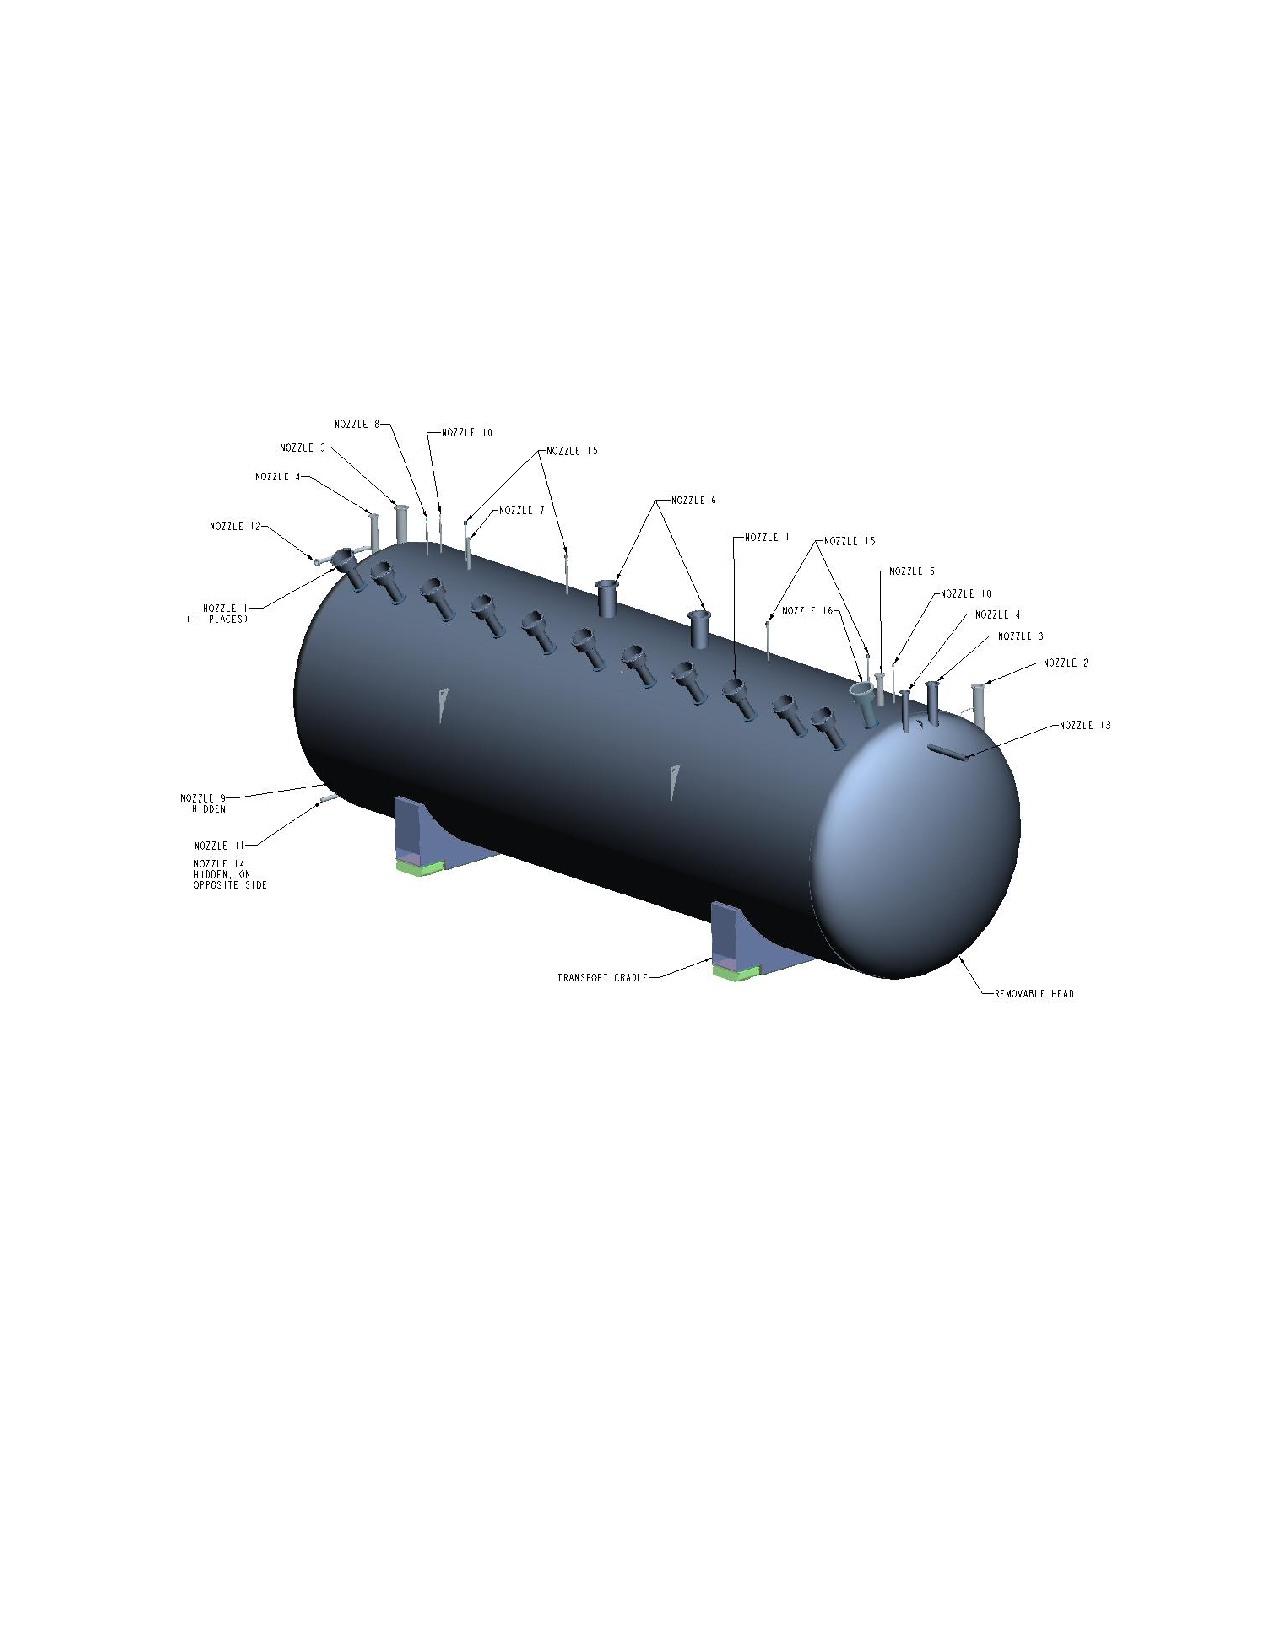
\includegraphics[width=\linewidth]{figures/cryostat_nozzles}
\caption{MicroBooNE cryostat with nozzle penetrations labeled.}
\label{fig:cryostat-drawing}
\end{figure}

\begin{figure}[htb]
\centering	
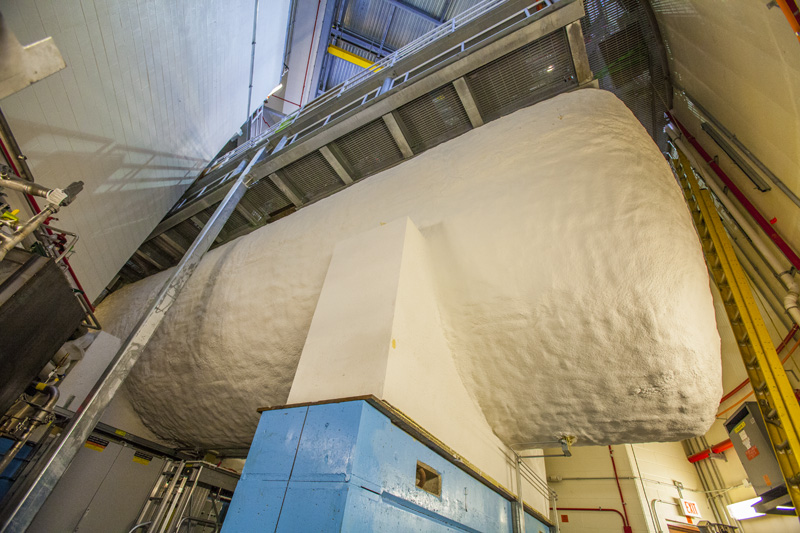
\includegraphics[width=0.45\linewidth]{figures/14-0222-03D.jpg}
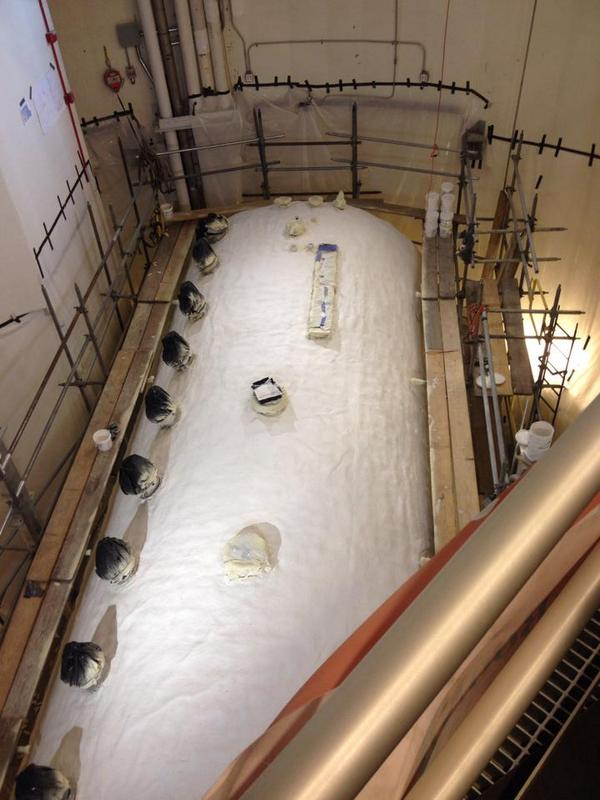
\includegraphics[width=0.45\linewidth]{figures/foam2.jpg}
\caption{Photographs of the cryostat after application of exterior foam insulation.}
\label{fig:cryostat-foam}
\end{figure}


The vessel surface has 34 nozzle penetrations for cryogenic and electrical services, detailed in table~\ref{tab:cryostat-feedthroughs}.  All nozzles are sealed with feedthroughs, flanges, or pipes that are suitable for operation at the nominal pressure and temperature of the cryostat.  

%\begin{}
\begin{table}[!htb]
   \centering
    \caption{List of nozzle penetrations in MicroBooNE cryostat.  CF=ConFlat flanges, RFWN=raised face weld neck flanges.} 
    \begin{tabular}{lcr} % Column formatting, @{} suppresses leading/trailing space
    \hline
    Nozzle ID & Function & Flange\\
    \hline
     N1A-N1K & \lartpc Signal Feedthrough & 14'' CF\\
     N2 & \lartpc HV Feedthrough & 8'' CF\\
     N3A-N3B & Purity Monitor & 8'' CF\\
     N4 & Temperature Signals & 6'' CF\\
     N5 & Safety Vent & 4'' RFWN\\
     N6A-N6B & Vacuum Pump-Out & 10'' RFWN\\
     N7 & Condensor & 3''\\
     N8 & Top Instrument Port & 3/4''\\
     N9 & Bottom Instrument Port & 3/4''\\
     N10A-N10B & Liquid Level Probe & 3/4''\\
     N11 & Gas Circulation In & 2''\\
     N12 & Gas Circulation Out & 2''\\
     N13 & From LAr Filters & 3''\\
     N14 & To LAr Pumps & 2''\\
     N15A-N15B & Laser Calibration & 2-3/4'' CF \\
     N16 & PMT Signal Feedthrough & 14'' CF\\
     N17 & Spare & 6'' CF\\
     N18 & Temperature Signals & 6'' CF\\
     N19 & Spare & 6'' CF\\
                  \hline
   \end{tabular}
   \label{tab:cryostat-feedthroughs}
\end{table} 



\subsection{Liquid Argon Purification Subsystem}
\label{sec:purification}

The heart of the cryogenic system is the liquid argon purification subsystem.  The primary requirement of this subsystem is to keep the level of electronegative contamination to below 100 ppt of oxygen-equivalent contaminants.  This requirement was determined by the physics needs of the experiment, namely the need to keep the attenuation of ionization electrons to less than 20\% over the longest drift distance in the LArTPC.  In addition to the requirement on the electronegative contamination, the system must maintain the level of nitrogen contamination in the argon at less than 2 parts per million (ppm) \cite{Jones:2013bca} to keep the attenuation of the scintillation photons in the argon to a minimum.  

The MicroBooNE argon purification subsystem consists of liquid argon pumps and filters that serve to circulate the argon and remove impurities that degrade the quality of the data collected by the active detectors.  There are two pumps in the system arranged in parallel in order to allow for continuous recirculation while one pump is being serviced.  Similarly, there are two sets of filters arranged in parallel in the system.  Figure \ref{flowdiagram} schematically depicts the flow of liquid and gaseous argon in the MicroBooNE cryogenic system.

\begin{figure}
\centering 
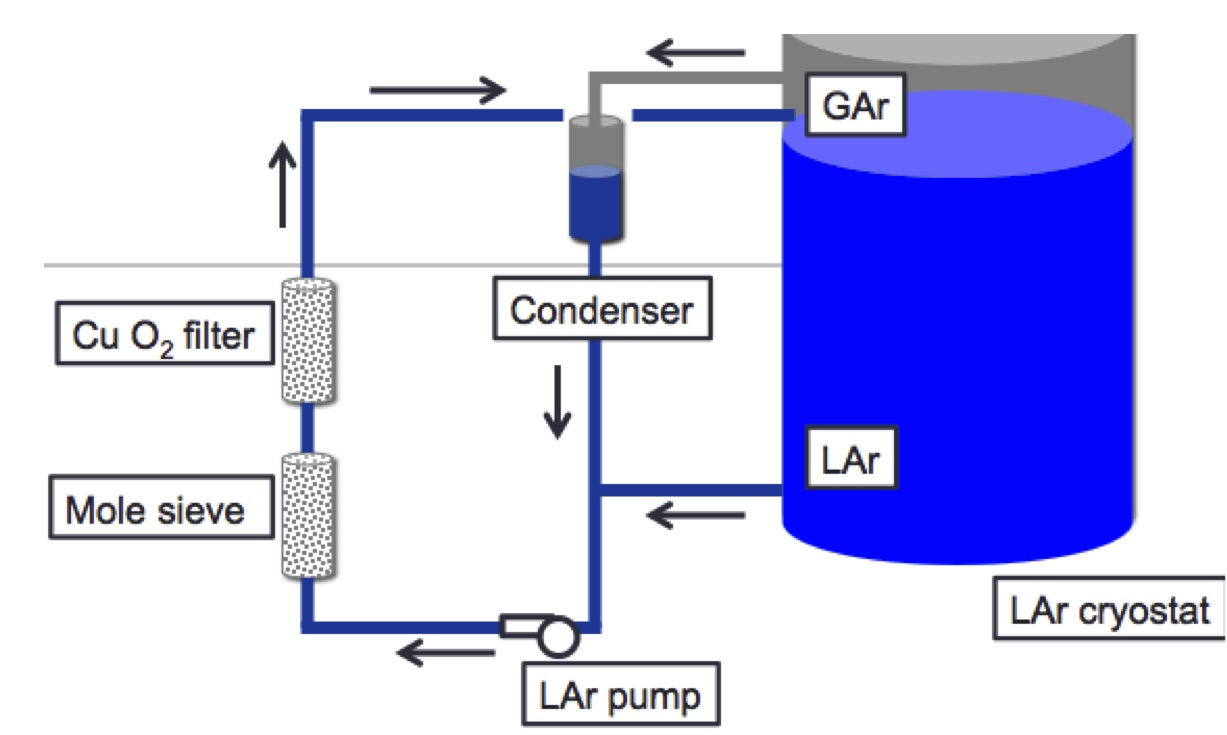
\includegraphics[width=0.45\textwidth]{figures/flow_diagram.jpg}
\caption{Flow diagram of argon in MicroBooNE, showing direction of liquid and gaseous argon in the cryogenic system.  Gaseous argon from the cryostat is condensed and directed through the purification subsystem. Liquid argon drawn from the cryostat volume is directed into the purification subsystem.  \textbf{NOTE: Update with better figure!}}
\label{flowdiagram}
%%NOTE:  Need a figure for this. - MPS, June 30, 2015
\end{figure}


%\subsubsubsection{Recirculation Pumps}

The recirculation pumps are Barber-Nichols~\cite{barber-nichols} BNCP-32B-000 magnetically-driven partial-emission centrifugal pumps.  Each pump isolates the liquid argon from the electric motor.  The impeller, inducer, and driving section of the magnetic coupling each have their own bearings that are lubricated by the liquid argon at the impeller.  The motor is controlled by a variable frequency drive (VFD) that allows adjustment of the pump speed to produce the desired head pressure and flow within the available power range of the motor.    

%\subsubsubsection{Filter Skids}

Each filter skid contains two filters, each having identically-sized filtration beds of 77~liters.  The first filter that the argon stream enters contains a 4A molecular sieve supplied by Sigma-Aldrich~\cite{sigma-aldrich} that primarily removes water contamination but can also remove small amounts of nitrogen and oxygen.  The second filter contains BASF~CU-0226~S, a highly-dispersed copper oxide impregnated on a high-surface-area alumina, which removes oxygen~\cite{basf} and, to a lesser extent, water.  Thus, the oxygen filter is placed downstream of the molecular sieve to maximize oxygen filtration.  The oxygen-filtering media must be reduced to copper with the procedure described below before it can remove oxygen from the liquid argon.  The filters are insulated with vacuum jackets and aluminum radiation shields.  The metallic radiation shields were chosen because the filter regeneration temperatures, described below, would damage traditional aluminized mylar insulation.  Pipe supplying the filter regeneration gas is insulated both inside the filter vacuum-insulation space and outside the filter with Pyrogel XT which is an aerogel-based insulation~\cite{aspen-aerogels} that can withstand temperatures up to $650^{\circ}{\rm C}$. 

The filters are regenerated {\it in situ} using heated gas, by a procedure developed for LAPD.  The filters are regenerated using a flow of argon gas that is heated to $200^{\circ}{\rm C}$, supplied by a commercial 500~liter liquid argon dewar.   Once the argon gas reaches $200^{\circ}{\rm C}$, a small flow of hydrogen is mixed into the primary argon flow and exothermically combines with oxygen captured by the filter to create water.  Too much hydrogen mixed in with the primary argon flow would induce temperatures that are sufficiently high to damage the copper-based filter media.  The damage is induced by sintering of the copper, which reduces the available filter surface area.  Thus, precautions are taken to maintain a hydrogen fraction below 2.5\% of the heated gas mixture.  During the heated gas regeneration, five filter-bed temperature sensors monitor the filter-material temperature and the water content of the regeneration exhaust gas is measured.  To remove any remaining trace amounts of water, the filters are then evacuated using turbomolecular vacuum pumps while they cool. 

A particulate filter with an effective filtration of 10 microns, positioned between the cryostat and the filter skids, prevents any debris in the piping from being introduced into the cryostat.  The particulate filter consists of a commercial stainless steel sintered-metal cylinder mounted in a custom cryogenic housing and vacuum jacket.  Filtration is accomplished by flowing liquid argon to the interior, then outward through the walls, of the sintered-metal cylinder.  Flanges on the argon piping, along with flanges and edge-welded bellows on the vacuum jacket, allow removal of the particulate filter.  

\begin{figure}
\centering 
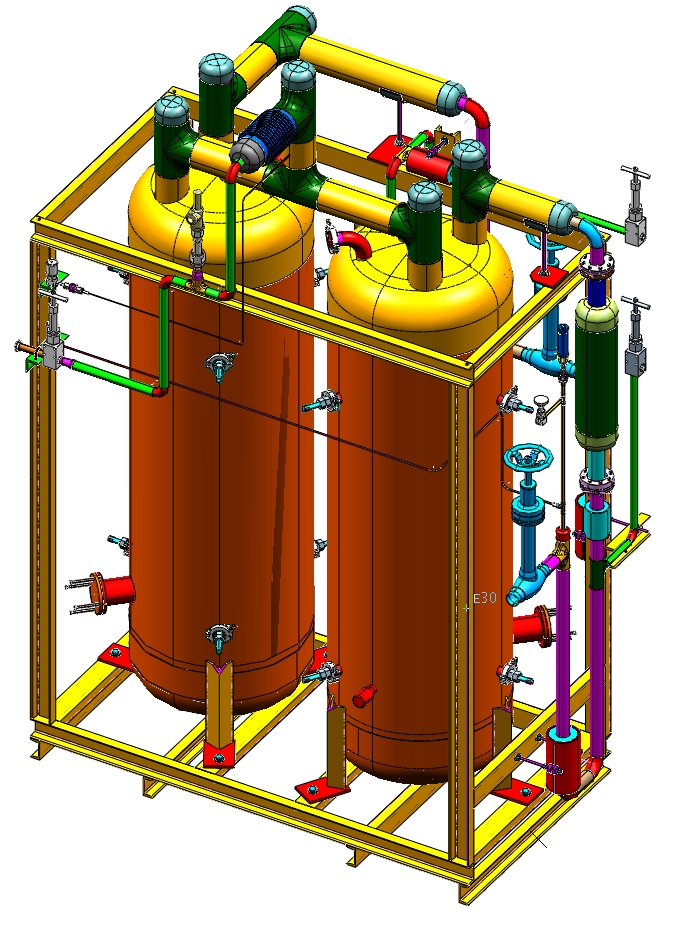
\includegraphics[width=0.45\textwidth]{figures/cryo-filter-skid}
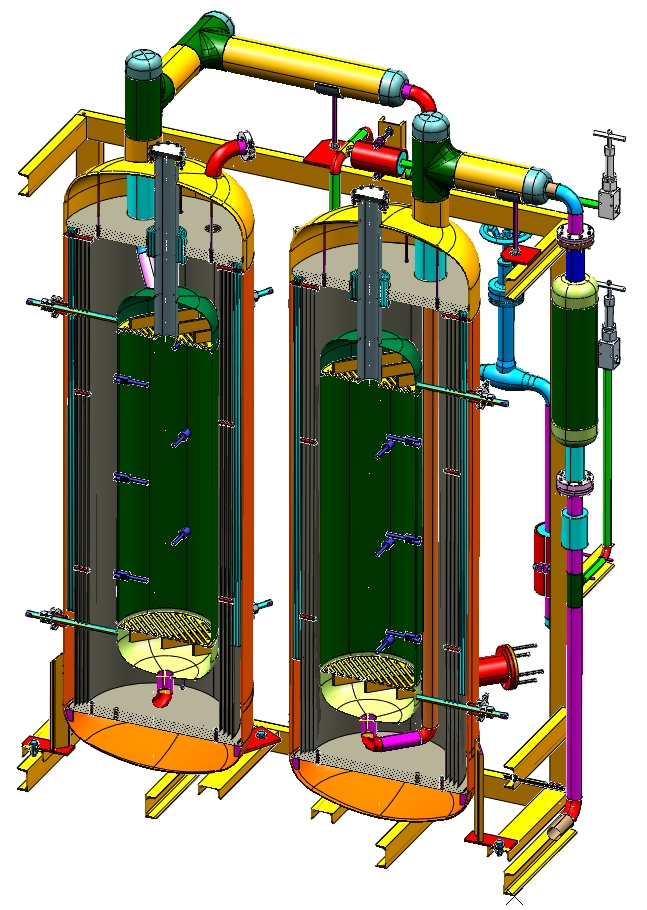
\includegraphics[width=0.45\textwidth]{figures/cryo-filter-skid-cutaway}
\caption{Three-dimensional rendering of a MicroBooNE filter skid.  The left drawing shows the full skid, while the right drawing shows a cut-away of the vessels.}
\label{filters}
\end{figure}


%\subsubsubsection{Piping and Valves}

The argon-purification piping is 2.54~cm diameter stainless steel that was pre-insulated by the manufacturer with 10.2~cm of polyurethane foam.  During the fabrication process, all piping was washed with distilled water and detergent to remove oil and grease, then cleaned with ethanol.  All valves associated with the argon-purification piping utilize a metal seal with respect to ambient air, either through a bellows or a diaphragm, to prevent the diffusion of oxygen and water contamination.  The exhaust side of each relief valve is continuously purged with argon gas to prevent diffusion of oxygen and water from ambient air across the o-ring seal.  Where possible, ConFlat flanges with copper seals are used on both cryogenic and room-temperature argon piping.  Pipe flanges in the system are sealed using spiral-wound graphite gaskets.  Smaller connections are made with VCR fittings with stainless steel gaskets.  

\subsection{Nitrogen Refrigeration}

The cryostat and purification systems that contain the liquid argon are subject to heat load from the environment, as well as from the active detectors that have electrical power enabled.  To keep these systems operating at a stable temperature and pressure, a liquid nitrogen refrigeration system is present to provide the necessary cooling power.  The liquid nitrogen system contains two condensers that are arranged in parallel.  One of these is utilized for normal operations and one serves as a backup on standby.  Each condenser contains two liquid nitrogen coils, an inner and an outer, with the gas argon on the shell side, as shown in figure~\ref{fig:condenser}.  Typically only one coil is actively running and the second can be manually activated during situations where the system heat load is higher than usual.  Each condenser is sized to handle a heat load of approximately 9.5 kW.  With the vessel full of liquid argon and no pump or liquid argon circulation running, the condenser uses 600-650 gallons of liquid nitrogen per day, which equates to a 3.9 kW system heat load.  Once liquid argon begins circulating using the pumps, this usage rate will increase by 50-100$\%$.

\begin{figure}[htb]
\centering	
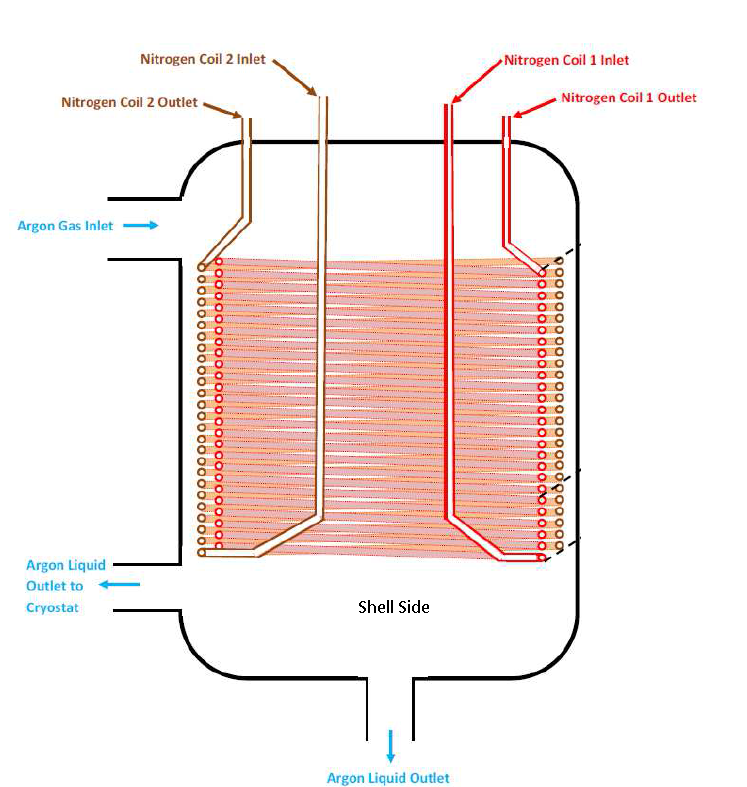
\includegraphics[width=0.75\linewidth]{figures/condenser.png}
\caption{Diagram of a condenser.}
\label{fig:condenser}
\end{figure}



\subsection{Controls and Purity Monitoring}

MicroBooNE makes use of resistive thermal devices (RTDs) to measure temperatures throughout the experimental infrastructure. Twelve RTDs are located along the walls of the cryostat, and another ten RTDs are mounted inside screws attached to the structure of the LArTPC. Each of the filter vessels in the purification system contain nine RTDs. The RTDs within the filter vessels prevent overheating which could potentially occur during filter regeneration with heated argon-hydrogen gas.

Liquid argon contaminations ranging between 300 and 50~ppt oxygen equivalent can be measured using double-gridded ion chambers, henceforth referred to as purity monitors, immersed in liquid argon. The design of the purity monitors is based on the design presented in Ref.~\cite{Carugno:1990-purityMonitor}.  Reference~\cite{Adamowski:2014-LAPD} gives a thorough description of the purity monitors, the data-acquisition hardware and software used in LAPD. MicroBooNE uses the same type of purity monitors, and the same data-acquisition hardware and software. 

A measure of the electronegative impurities is made with the purity monitor by examining the fraction of electrons generated at the purity monitor cathode that subsequently arrive at the purity monitor anode $(Q_A/Q_C)$ after a drift time $t$. The ratio of $(Q_A/Q_C)$ is related to electron lifetime, $\tau$, such that

\begin{equation}
Q_A/Q_C = e^{-t/\tau}.
\end{equation}

Measurement of liquid argon purity in the MicroBooNE cryogenic system are provided by three purity monitors of varying lengths. One purity monitor with a drift distance of 50~cm sits in a vessel just downstream of the filters and is used to monitor filter effectiveness. Two purity monitors, one with a drift distance of 19~cm and the other with a drift distance of 50~cm, sit within the primary MicroBooNE vessel at each end of the LArTPC.


 

